\documentclass[tikz, margin=2mm,convert={density=300,size=1920x1080,outext=.png}]{standalone}

\usepackage{xcolor}

\newcommand{\len}{7}% x direction
\newcommand{\bre}{7}% y direction
\newcommand{\hei}{4}% z direction
\newcommand{\frontcolor}{black!15!white}
\newcommand{\topcolor}{black!30!white}
\newcommand{\sidecolor}{black!45!white}

\begin{document}
    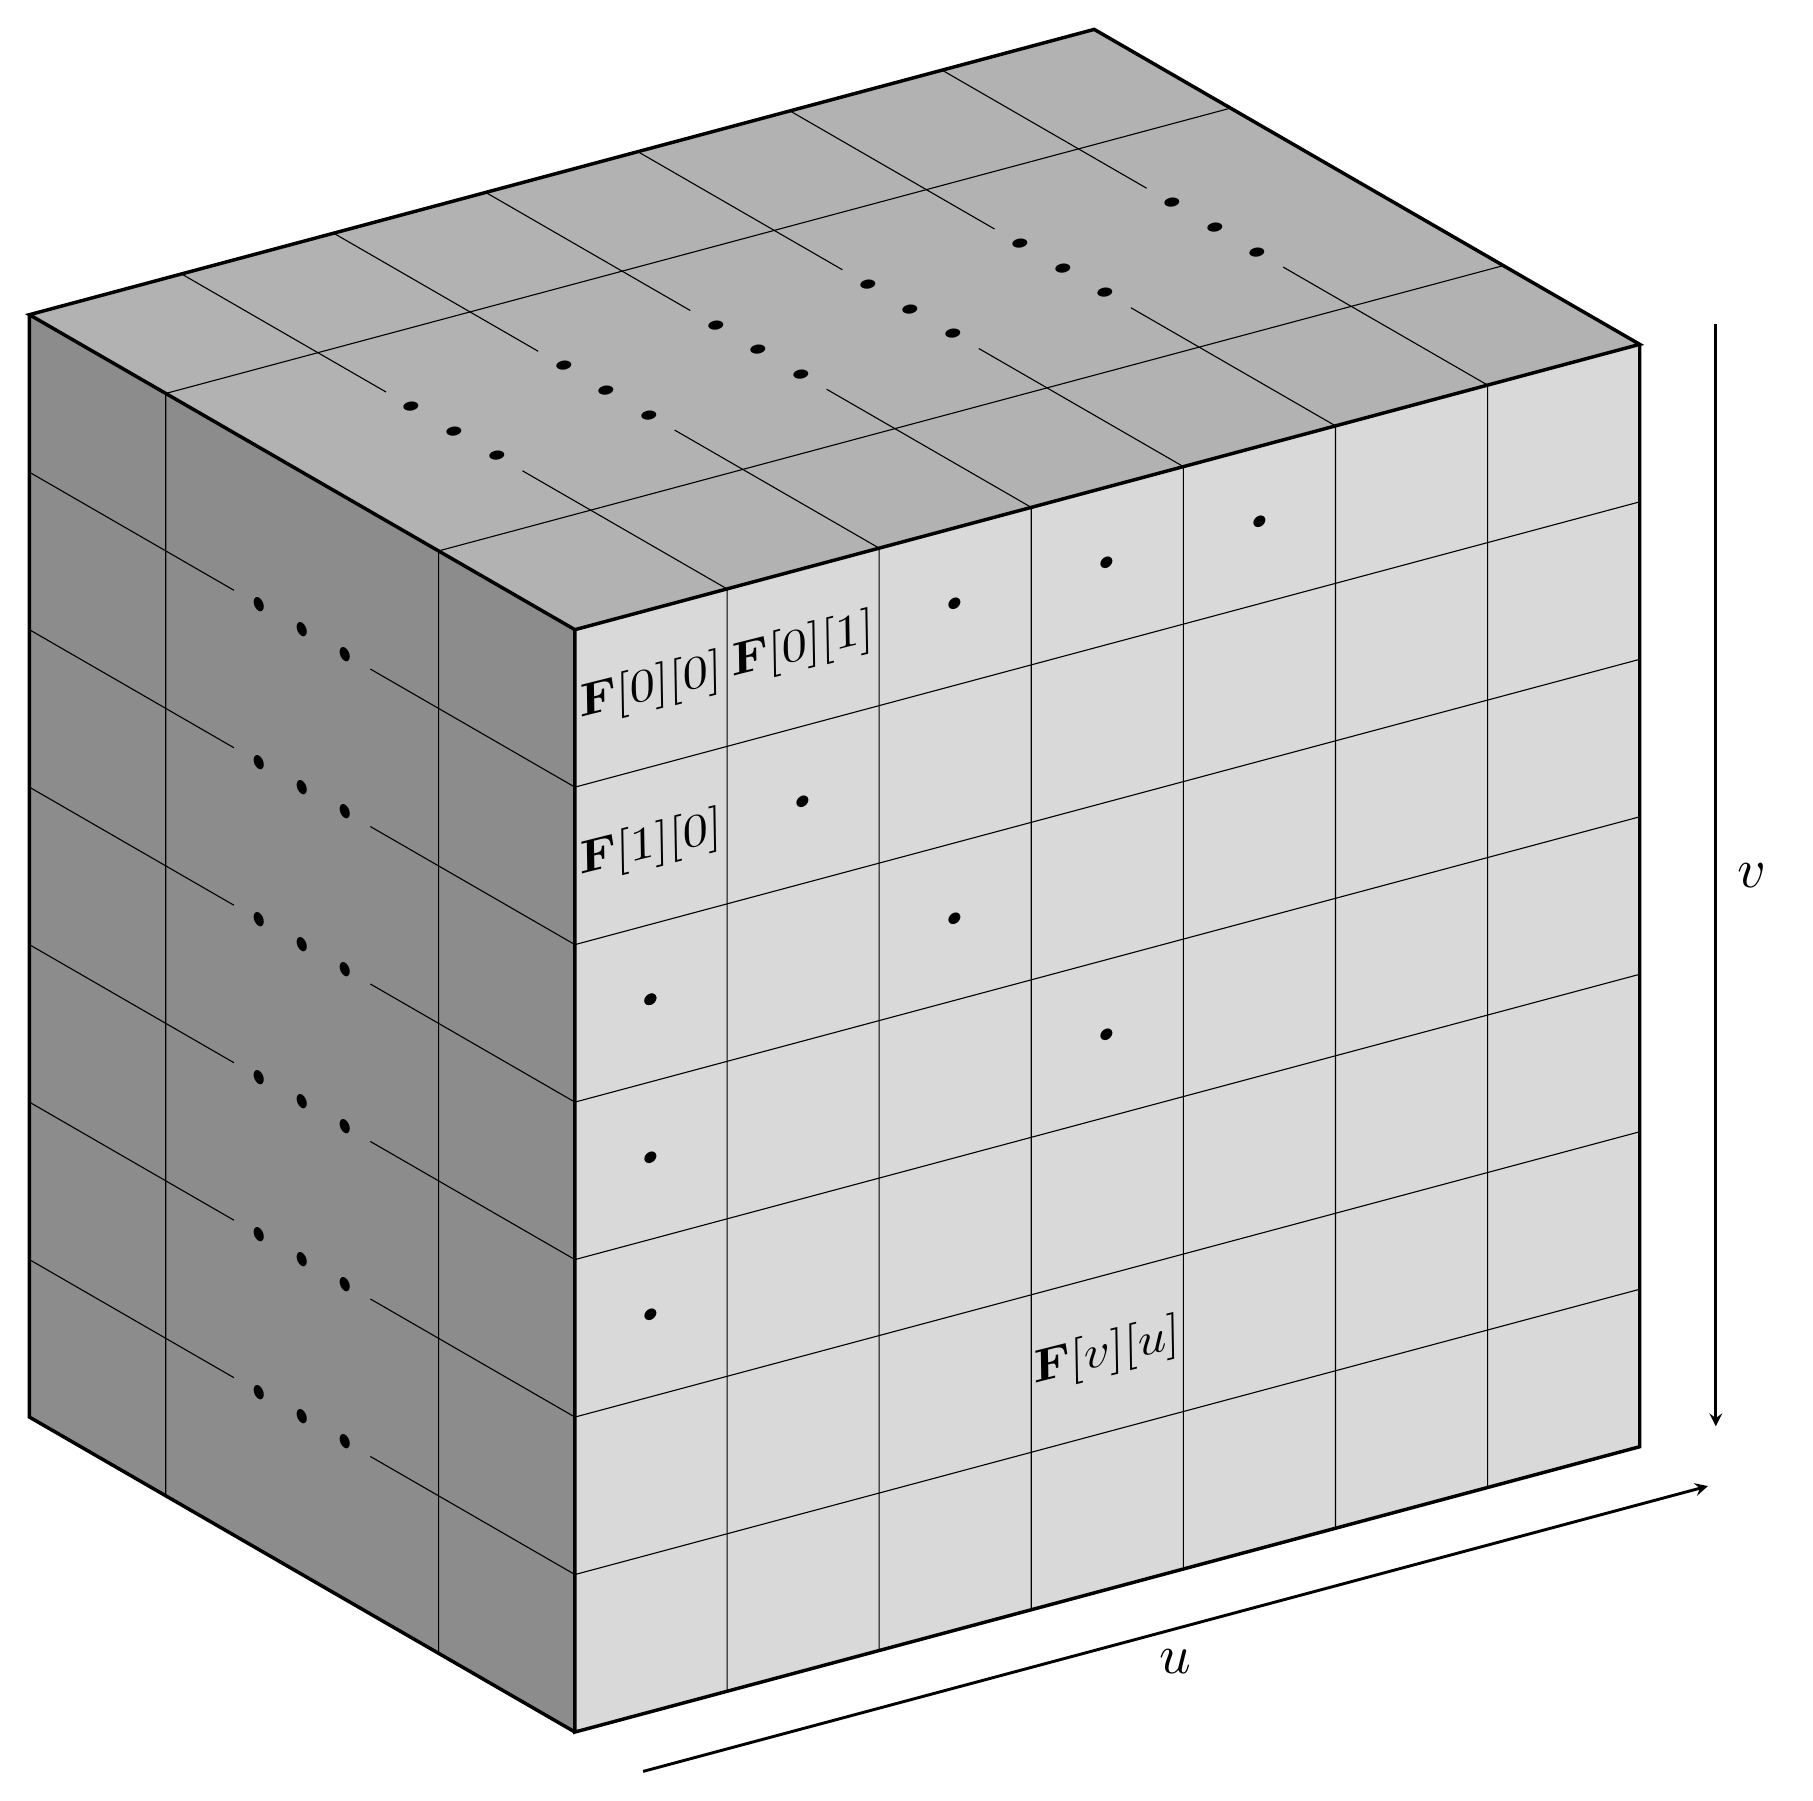
\begin{tikzpicture}[x=(15:2cm), y=(90:2cm), z=(330:2cm), >=stealth]
        \coordinate (O) at (0, 0, 0);
        \coordinate (A) at (\len, 0, 0);
        \coordinate (B) at (0, \bre, 0);
        \coordinate (C) at (\len, \bre, 0);
        \coordinate (D) at (0, 0, \hei);
        \coordinate (E) at (\len, 0, \hei);
        \coordinate (F) at (0, \bre, \hei);
        \coordinate (G) at (\len, \bre, \hei);
        
        % color
        \fill[\frontcolor] (D) -- (E) -- (G) -- (F) -- cycle;
        \fill[\topcolor] (B) -- (C) -- (G) -- (F) -- cycle;
        \fill[\sidecolor] (O) -- (B) -- (F) -- (D) -- cycle;
        
        % draw dotted dividing lines
        \foreach \z in {1, 3}
            \draw[-] (0, 0, \z) -- (0, \bre, \z) -- (\len, \bre, \z); 
        \foreach \x in {1, ..., 6}{
            \draw[-] (\x, 0, \hei) -- (\x, \bre, \hei) -- (\x, \bre, \hei-1.5);
            \draw[-] (\x, \bre, 0) -- (\x, \bre, 1.5);
            \node at (\x, \bre, \hei/2) [scale=4, rotate=330, xslant=.5] {$\ldots$}; 
        }
        \foreach \y in {1, ..., 6}{
            \draw[-] (0, \y, \hei-1.5) -- (0, \y, \hei) -- (\len, \y, \hei);
            \draw[-] (0, \y, 0) -- (0, \y, 1.5);
            \node at (0, \y, \hei/2) [scale=4, rotate=330, xslant=-.5] {$\ldots$};
        }
        
        % box edges
        \draw[line width=1.25pt] (B) -- (F) -- (G) -- (C) -- cycle;
        \draw[line width=1.25pt] (F) -- (D) -- (E) -- (G);
        \draw[line width=1.25pt] (B) -- (O) -- (D);
        
        % dimension labels
        \draw [->, line width=1.05pt] (0, 0, \hei+.5)  -- (\len, 0, \hei+.5)   node [midway, below, scale=2] {$u$};
        \draw [->, line width=1.05pt] (\len+.5, \bre, \hei)  -- (\len+.5, 0, \hei)   node [midway, right, scale=2] {$v$};
        
        % labels on the faces
        \node [draw=none, sloped, xslant=.25, rotate=15, scale=1.75] at (0.5, \bre-.5, \hei){$\mathbf{F}[0][0]$};
        \node [draw=none, sloped, xslant=.25, rotate=15, scale=1.75] at (0.5, \bre-1.5, \hei){$\mathbf{F}[1][0]$};
        \node [draw=none, sloped, xslant=.25, rotate=15, scale=1.75] at (1.5, \bre-0.5, \hei){$\mathbf{F}[0][1]$};
        \node [draw=none, sloped, xslant=.25, rotate=15, scale=1.75] at (3.5, \bre-5.5, \hei){$\mathbf{F}[v][u]$};
        \foreach \x in {2.5, 3.5, 4.5}
            \node [draw=none, sloped, xslant=.25, rotate=15, scale=4] at (0.5, \bre-\x, \hei){$\cdot$};
        \foreach \x in {2.5, 3.5, 4.5}
            \node [draw=none, sloped, xslant=.25, rotate=15, scale=4] at (\x, \bre-.5, \hei){$\cdot$};
        \foreach \diag in {1.5, 2.5, 3.5}
            \node [draw=none, sloped, xslant=.25, rotate=15, scale=4] at (\diag, \bre-\diag, \hei){$\cdot$};
        \node [draw=none, sloped, xslant=.25, rotate=15, scale=4] at (0.5, \bre-2.5, \hei){$\cdot$};
    \end{tikzpicture}
\end{document}